\section{Various Measure}
\subsection{KL Divergence}
Definition:
$$D_\textrm{KL}(q(x)||p(x)) = \int q(x)\log \frac{q(x)}{p(x)}dx$$
\begin{itemize}
	\item Forward KL: 
	\begin{itemize}
		\item If $q(z)\rightarrow 0, \textrm{Forward KL}\rightarrow \infty$ 
		\item Zero avoiding for $q(z)$ 
	\end{itemize}
	\item Reverse KL:
	\begin{itemize}
		\item If $p(z)\rightarrow 0, \textrm{Reverse KL}\rightarrow \infty$ 
		\item Zero forcing: $q(z)\rightarrow 0$ 
	\end{itemize}
\end{itemize}

Typically, $p(x)$ and $q(x)$ are far apart at the initial state. 

\begin{figure}[h]
	\begin{center}
		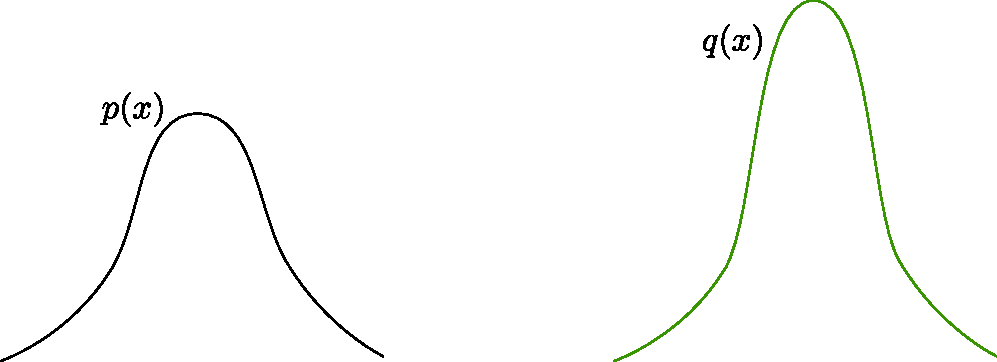
\includegraphics[scale=0.5]{./images/twodist.pdf}
	\end{center}
	\caption{Two distributions: $p(x)$ and $q(x)$}
	\label{fig:}
\end{figure}

Thus, both the forward KL and the reverse KL suffers an unstability issue. Specifically, in each case, if the denominator goes to zero, then the divergence goes to infinity. 

\subsection{Jensen-Shannon Divergence}

Definition:
$$D_{JS}(p_{data}||p_{G}) = \frac{1}{2}\Bigg[D_{KL}\Big(p_{data}\Big|\Big|\frac{p_{data}+p_{G}}{2}\Big)+D_{KL}\Big(p_{G}\Big|\Big|\frac{p_{data}+p_{G}}{2}\Big)\Bigg]$$

The KL divergence's issue can be alleviated by JS-divergence. Consider a simple example in Fig. \ref{fig:wassersteinexample}6
\begin{align*}
	\forall (x, y) \in P, x = 0 \text{ and } y \sim U(0, 1)\\
	\forall (x, y) \in Q, x = \theta, 0 \leq \theta \leq 1 \text{ and } y \sim U(0, 1)
\end{align*}

\begin{figure}[h]
	\begin{center}
		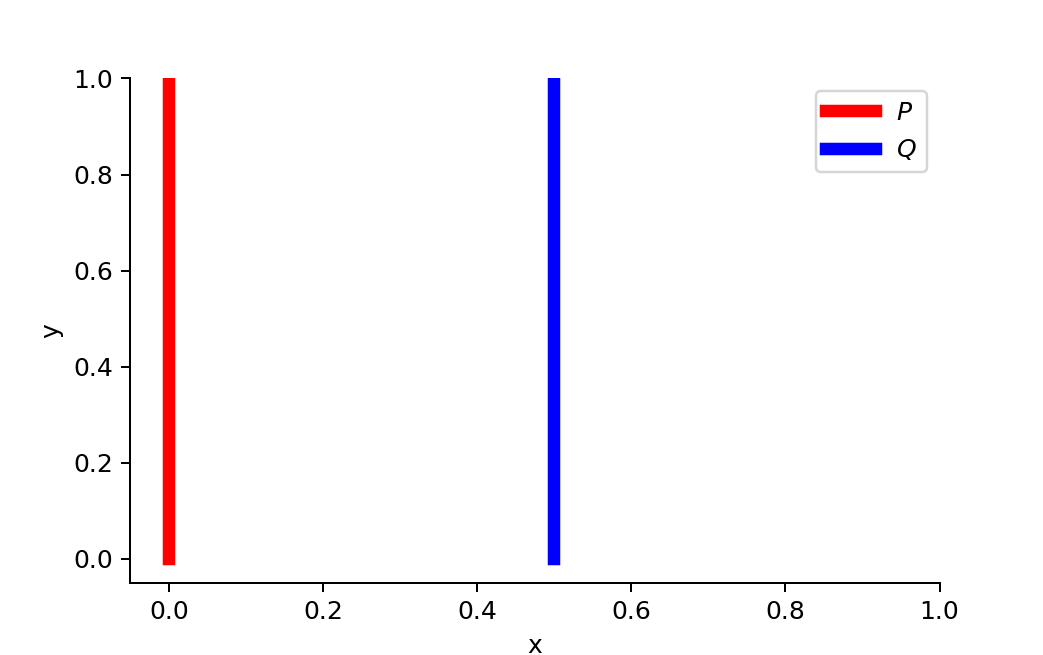
\includegraphics[scale=0.25]{./images/wassersteinexample.png}
	\end{center}
	\caption{Two distributions: $p(x)$ and $q(x)$}
	\label{fig:wassersteinexample}
\end{figure}

\begin{align*}
	D_\textrm{KL}(q(x)||p(x)) &= \infty\\
	D_\textrm{KL}(p(x)||q(x)) &= \infty\\
	D_{JS}(p_{data}||p_{G}) &= \frac{1}{2}\Bigg[D_{KL}\Big(p_{data}\Big|\Big|\frac{p_{data}+p_{G}}{2}\Big)+D_{KL}\Big(p_{G}\Big|\Big|\frac{p_{data}+p_{G}}{2}\Big)\Bigg]\\
	& = \frac{1}{2}\Bigg[D_{KL}\Big(p_{data}\Big|\Big|\frac{p_{data}}{2}\Big)++D_{KL}\Big(p_{G}\Big|\Big|\frac{p_{G}}{2}\Big)\Bigg]\\
	& = \frac{1}{2}[\log 2 + \log 2] = \log 2\\
	W(p,q) & = |\theta|
\end{align*}
Therefore, Jensen-Shannon divergence is more stabler than KL divergece. This is one of the reasons why GAN, which uses JS divergence works better than VAE, which uses KL divergence. 

However, JS divergence also has some problem. If the value is close to $\frac{1}{2}\log 2$, then the gradient will be very small or close to zero, because the divergence is close to constant. It means that a training speed is very slow. Thus, we need a better metric. 

\subsection{Wasserstein Distance}
Wasserstein Distance is a measure of the distance between two probability distributions. It is also called Earth Mover’s distance, short for EM distance, because informally it can be interpreted as the minimum energy cost of moving and transforming a pile of dirt in the shape of one probability distribution to the shape of the other distribution.
\begin{equation*}
	W(p_r, p_g) = \inf_{\gamma \sim \Pi(p_r, p_g)} \mathbb{E}_{(x, y) \sim \gamma}[\| x-y \|]
\end{equation*}

\begin{itemize}
	\item $\Pi$: is the transportation plan and the set of all possible joint probability distributions between $p_r$ and $p_g$. One joint distribution $\gamma \sim \Pi(p_r, p_g)$ describes one transport plan.\
	\item $\mathbb{E}_{x, y \sim \gamma} \| x-y \| = \sum_{x, y} \gamma(x, y) \| x-y \|$
	\item Finally, we take the minimum one among the costs of all dirt moving solutions as the EM distance (by infimum). 
\end{itemize}


